\newpage
\section[Fourier Reihen]{Fourier Reihen}
\textit{Die Fourier-Reihe ist ein wichtiges Instrument in der Physik, das uns ermöglicht (quasi-)periodische Funktionen mit einer Summe von vielen $\sin(x)$ und $\cos(x)$ zu approximieren.}
\subsection{Fourier-Reihe}\label{ssec:Fourier}


\begin{Def}{Fourier-Koeffizient}
Sei $f:\R \rightarrow \C$ eine $2\pi$-periodische Funktion. Die komplexe Zahl
$$c_k=\frac{1}{2\pi}\int_0^{2\pi}f(x)e^{-ikx}dx$$
heißt das k-te \red{Fourier-Koeffizient}.
\end{Def}
\begin{Def}{Fourier-Reihe}
Die Reihe $$F(f)=\sum_{k=-\infty}^\infty c_ke^{-ikx}$$ heißt die \red{Fourier-Reihe} von $f$
\end{Def}
\begin{Beispiel}{Beispiel einer Fourier-Reihe}
Gegeben sei die Funktion $$f(x)=\begin{cases}1 & \mbox{wenn $0< x\leq \pi$}\\
0 & \mbox{wenn $\pi< x\leq 2\pi$}
\end{cases}$$
Wir wollen nun die Fourier-Reihe zu der $2\pi$-periodischen $f$ bestimmen, um die Funktion zu approximieren. Wir berechnen zuerst $c_0$.
$$c_0=\frac{1}{2\pi}\int_0^\pi 1 e^{0} dx + \frac{1}{2\pi}\int_\pi^{2\pi} 0 e^{0} dx = \frac{1}{2\pi}\pi - 0 = \frac{1}{2}$$
Nun berechnen wir $c_1$, um ein Gefühl zu entwickeln.
$$c_1=\frac{1}{2\pi}\int_0^\pi 1 e^{-ix}dx + \frac{1}{2\pi}\int_0^\pi 0 e^{-ix}dx = \frac{1}{2\pi}\int_0^\pi  e^{-ix}dx = $$
$$=\frac{1}{2\pi} \int_0^\pi \cos(x) - i\sin(x) dx =\frac{1}{2\pi}([\sin(x)]^\pi_0+i[\cos(x)]^\pi_0)=\frac{1}{2\pi}(0-2i)=-\frac{i}{\pi}$$
Anschließend berechnen wir $c_k$.
$$c_k=\frac{1}{2\pi}\int_0^\pi 1 e^{-ikx}dx + \frac{1}{2\pi}\int_0^\pi 0 e^{-ikx}dx=\frac{1}{2\pi}\int_0^\pi 1 e^{-ikx}dx=$$
$$=\frac{1}{2\pi} [\frac{ie^{-ikx}}{k}]_0^{\pi}=\frac{1}{2\pi} [\frac{i(\cos(kx)-i\sin(kx))}{k}]_0^\pi=\begin{cases}-\frac{i}{\pi k} & \mbox{k ungerade}\\ 0 & \mbox{k gerade}\end{cases}$$
Die Fourier-Reihe der Funktion $f$ ist dann
$$F(f)=\frac{1}{2}-\frac{i}{\pi}e^{-ix}+\frac{i}{\pi}e^{ix}-\frac{i}{3\pi}e^{-3ix}+\frac{i}{3\pi}e^{3ix}-\frac{i}{5\pi}e^{-5ix}+\frac{i}{5\pi}e^{5ix}\dots$$
Dies könnte man noch umschreiben:
$$F(f)=\frac{1}{2}+\frac{2}{\pi}\sin(x)+\frac{2}{3\pi}\sin(3x)+\frac{2}{5\pi}\sin(5x)+\dots$$
\begin{center}
    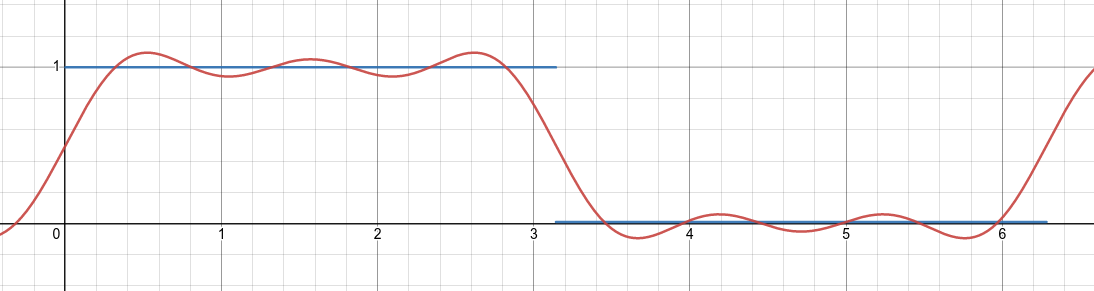
\includegraphics[width=.8\textwidth]{Dateien/Fourier_Beispiel.png}
\end{center}
Wie auf dem Bild zu sehen, approximieren wir mit jeden neuen Term die Funktion stückweise besser.

\end{Beispiel}
\begin{Satz}{Bemerkung}{Wichtige Fourier-Integrale}
Die folgenden Integrale sind sehr wichtig bei der Berechnung von Fourier-Reihen:
\begin{enumerate}
    \item $\int_0^{2\pi} \cos(kx)\sin(lx)dx=0, \mbox{ für $\forall k,l$}$
    \item $\int_0^{2\pi}\cos(kx)\cos(lx)dx=0 \mbox{ für $k\neq l$}$
    \item $\int_0^{2\pi}\sin(kx)\sin(lx)dx=0 \mbox{ für $k\neq l$}$
    \item $\int_0^{2\pi}\sin^2(kx)dx=\pi \mbox{ für $k\geq 1$}$
    \item $\int_0^{2\pi}\cos^2(kx)dx=\pi \mbox{ für $k\geq 1$}$
\end{enumerate}
\red{Wichtig!} Diese Beziehungen gelten nur für $k,l\in\N$.
\end{Satz}
\begin{Satz}{Bemerkung}{Fourier für un- und gerade Funktionen}
Es gilt $$F_n(f)=\frac{a_0}{2}+\sum_{k=1}^n (a_k\cos(kx)+b_k\sin(kx))$$
wobei $$a_k= c_k+c_{-k}=\frac{1}{\pi}\int_0^{2\pi}f(x)\cos(kx)dx$$
$$b_k=i(c_k-{c-k})=\frac{1}{\pi}\int_0^{2\pi}f(x)\sin(kx)dx$$
Wenn $f$ reellwertig ist, dann ist $c_{-k}=\overline{c_k}$ und $F_n(f)$ auch reellwertig. \\ \\
Ist $f$ gerade (d.h. $f(-x)=f(x)$), dann gilt
$$F_n(f)=\frac{a_0}{2}+\sum_{k=1}^n a_k\cos{(kx)}$$
Ist $f$ ungerade (d.h. $f(-x)=-f(x)$), dann gilt
$$F_n(f)=\sum_{k=1}^n b_k\sin{(kx)}$$
\end{Satz}
Eine weitere Anwendung der Fourier-Reihe ist auch das Beweisen von Folgen
\begin{Beispiel}{Folgenbeweise mit Fourier}
Wir sollen die Formel $\frac{\pi^2}{6}=1+\frac{1}{4}+\frac{1}{9}+\dots$ beweisen indem wir die Fourier-Reihe der $2\pi$-periodischen Funktion $f(x)=x^2$ im Intervall $-\pi\leq x\leq \pi$ bestimmen.
$$c_0=\frac{1}{2\pi}\int_{-\pi}^{\pi}x^2e^0dx=\frac{1}{2\pi}[\frac{x^3}{3}]_{-\pi}^{\pi}=\frac{1}{2\pi}(\frac{\pi^3}{3}+\frac{\pi^3}{3})=\frac{\pi^2}{3}$$
$$c_k=\frac{1}{2\pi}\int_{-\pi}^{\pi}x^2e^{-ikx}dx=\begin{cases} \frac{1}{k^2} & \mbox{wenn $k$ gerade} \\
-\frac{1}{k^2} & \mbox{wenn $k$ ungerade}
\end{cases}$$
$$F_n(f)=\frac{\pi^2}{3}-2\cos(x)+\frac{1}{2}\pi\cos(2x)-\frac{2}{9}\cos(3x)+\dots$$
Nun setzen wir für $x$ den Wert $x=\pi$ ein und erhalten:
$$F_n(f(\pi))=\frac{\pi^2}{3}+2+\frac{1}{2}+\frac{2}{9}+\dots$$
Wir wissen, dass $f(\pi)=\pi^2$ und substrahieren $\frac{\pi^2}{3}$ von beiden Seiten
$$\frac{\pi^2}{3}=2+\frac{1}{2}+\frac{2}{9}+\dots$$
Nun teilen wir beide Seiten mit $2$ und erhalten
$$\frac{\pi^2}{6}=1+\frac{1}{4}+\frac{1}{9}+\dots$$
\end{Beispiel}




\subsection{Konvergenz der Fourier Reihe}\label{ssec:FourierKonv}
\begin{Def}
{$L^2$-Halbnorm}
Sei $V$ der Vektorraum der $2\pi$-periodischen Funktionen $f:\R \rightarrow \C$, wobei $f$ Riemann-integrierbar ist. Dann ist die Hermitische Form 
$$||f||_2=\langle f,f\rangle = \frac{1}{2\pi}\int_0^{2\pi}f(x)\overline{f(x)}dx, \space f\in V$$
die \red{$L^2$-Halbnorm} von $f$.
\end{Def}
\begin{Satz}{Satz}{Konvergenz der Fourier-Reihe im quadratischen Mittel}
Sei $V$ der Vektorraum der $2\pi$-periodische Funktionen $f:\R\rightarrow\C$, für die $f$ integrierbar ist. \\
i) Für $\forall f\in V$ gilt
$$||f||_2^2=\sum_{k=-\infty}^\infty |c_k|^2$$
ii) Die Fourier-Reihe von $f\in V$ konvergiert im quadratischen Mittel gegen $f$, d.h. $\lim_{n\rightarrow \infty}||f-F_n(f)||_2=0$.
\end{Satz}
Es gibt tatsächlich keine $2\pi$-periodische Funktion im $\mathcal{L}^2$, dessen Fourier-Reihe nicht fast überall gegen $f$ konvergieren würde.